\documentclass[compress,table]{beamer}


\usepackage{tikz} % Pretty pictures, google tikzmanual.pdf
\usetikzlibrary{arrows,decorations.pathmorphing,decorations.markings}
\usetikzlibrary{shapes,decorations.pathreplacing,backgrounds}
\usetikzlibrary{matrix}

\usepackage{pgfplots}
%\pgfplotsset{compat=1.9}

\tikzstyle{vecArrow} = [thick, decoration={markings,mark=at position
   1 with {\arrow[semithick]{open triangle 60}}},
   double distance=1.4pt, shorten >= 5.5pt,
   preaction = {decorate},
   postaction = {draw,line width=1.4pt, white,shorten >= 4.5pt}]
\tikzstyle{innerWhite} = [semithick, white,line width=1.4pt, shorten >= 4.5pt]

\usetikzlibrary{patterns}


\newcommand{\nullNode}{\node[circle,fill=white,minimum width={width("1")},minimum height={height("1")}]}

\newcommand{\posNode}{\node[circle,draw,fill=red!30,minimum width={width("1")},minimum height={height("1")}]}
\newcommand{\posStop}[1]{\node[regular polygon,regular polygon sides=3,draw,fill=red!70] at (#1) {} }


\newcommand{\negNode}{\node[rectangle,draw,fill=blue!30,minimum width={width("1")},minimum height={height("1")}]}
\newcommand{\negStop}[1]{\node[regular polygon,regular polygon sides=3,draw,fill=blue!70] at (#1) {} }

\newcommand{\com}[1]{\draw[draw,fill=yellow] (#1) circle (10pt) }
\newcommand{\query}[1]{\node[draw,diamond,fill=gray!50] at (#1) {$???$}}


\newcommand{\fillRed}{\draw[preaction={fill=red}, pattern=north west lines, pattern color=white]}
\newcommand{\fillGreen}{\draw[preaction={fill=green}, pattern=horizontal lines, pattern color=black]}
\newcommand{\fillYellow}{\draw[preaction={fill=yellow}, pattern=north east lines, pattern color=citrine]}
\newcommand{\fillBlue}{\draw[preaction={fill=blue}, pattern=crosshatch, pattern color=gray]}
\newcommand{\fillGray}{\draw[preaction={fill=gray}]}

\usepackage{amsmath}
\usepackage{eepic}
\usepackage{epic}
\usepackage{epsfig}
\usepackage{moreverb}
\usepackage{stfloats}
\usepackage{algorithm}
\usepackage{amsthm}
\usepackage{algpseudocode}
\usepackage{amsthm}
\usepackage{multicol}
\usepackage{colortbl}
\usepackage{rotating}

\usetheme{Warsaw}
\usepackage{multicol}

\colorlet{mycolor}{orange!80!black}% change this color to suit your needs
\definecolor{citrine}{rgb}{0.89, 0.82, 0.04}

\AtBeginSection[]{
  \setbeamercolor{section in toc shaded}{use=structure,fg=structure.fg}
  \setbeamercolor{section in toc}{fg=mycolor}
  \setbeamercolor{subsection in toc shaded}{fg=black}
  \setbeamercolor{subsection in toc}{fg=mycolor}
  \frame<beamer>{
    \begin{multicols}{2}
      \frametitle{Outline}
      \setcounter{tocdepth}{2}  
      \tableofcontents[currentsection,subsections]
    \end{multicols} 
  }
}

\setbeamercolor{author in head/foot}{fg=white}
\setbeamercolor{title in head/foot}{fg=mycolor}
\setbeamercolor{section in head/foot}{fg=mycolor}
\setbeamertemplate{section in head/foot shaded}{\color{white!70!black}\insertsectionhead}
\setbeamercolor{subsection in head/foot}{fg=mycolor}
\setbeamertemplate{subsection in head/foot shaded}{\color{white!70!black}\insertsubsectionhead}
\setbeamercolor{frametitle}{fg=white}
\setbeamercolor{framesubtitle}{fg=white}

\title{One Dimensional Algorithmic Questions}
\author{James Zuber}
\institute{Stony Brook University}
\date{\today}

\begin{document}

\begin{frame}
  \maketitle
\end{frame}

\section[Airplane Seating]{Airplane Seating}
\begin{frame}\frametitle{1-Dimensional Airplanes}

\begin{figure}[H]
\label{fig:lineplane}
\centering
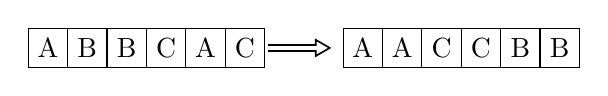
\begin{tikzpicture}[scale=1]
\draw (0,0.0) +(-.25,-.25) rectangle ++(.25,.25);
\draw (0,0.0) node{A};
\draw (0.5,0) +(-.25,-.25) rectangle ++(.25,.25);
\draw (0.5,0) node{B};
\draw (1.0,0) +(-.25,-.25) rectangle ++(.25,.25);
\draw (1.0,0) node{B};
\draw (1.5,0) +(-.25,-.25) rectangle ++(.25,.25);
\draw (1.5,0) node{C};
\draw (2.0,0) +(-.25,-.25) rectangle ++(.25,.25);
\draw (2.0,0) node{A};
\draw (2.5,0) +(-.25,-.25) rectangle ++(.25,.25);
\draw (2.5,0) node{C};

\visible<2-3>
{
\draw[vecArrow] (2.8,0) to (3.6,0);

\draw (4,0.0) +(-.25,-.25) rectangle ++(.25,.25);
\draw (4,0.0) node{A};
\draw (4.5,0) +(-.25,-.25) rectangle ++(.25,.25);
\draw (4.5,0) node{A};
\draw (5.0,0) +(-.25,-.25) rectangle ++(.25,.25);
\draw (5.0,0) node{C};
\draw (5.5,0) +(-.25,-.25) rectangle ++(.25,.25);
\draw (5.5,0) node{C};
\draw (6.0,0) +(-.25,-.25) rectangle ++(.25,.25);
\draw (6.0,0) node{B};
\draw (6.5,0) +(-.25,-.25) rectangle ++(.25,.25);
\draw (6.5,0) node{B};
}
\end{tikzpicture}
\end{figure}

\visible<3>
{
Important features:

\begin{itemize}
\item Airplane only has 1 long row of seats.
\item All family members identical.
\item No preferred sort order (ABC as good as CAB).
\item Can only swap 2 passengers at a time.
\end{itemize}
}
\end{frame}

\begin{frame}\frametitle{Hardness}
Given a set of $n = 3m$ integers $x_i$, is there a grouping of the $x_i$ into $m$ disjoint triplets so that the sum of each triplet is the same number $k$?  

Gadgets:
\visible<2->
{
Large blocking families $B_j$ between each $k$-width seating area.
}

\visible<3->
{
One family, $f_i$ for each $x_i$. $|f_i| = x_i$
}

\visible<4->
{
One seatwarmer family $S$ at end of plane.
}


Starting position:

\begin{figure}[H]
\centering
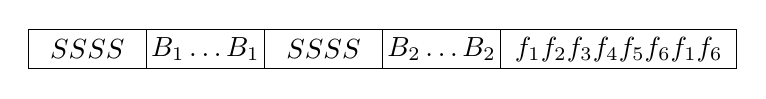
\begin{tikzpicture}[scale=1]
\draw (0,0.0) +(-.75,-.25) rectangle ++(.75,.25);
\visible<4->
{
\draw (0,0.0) node{$SSSS$};
}
\draw (1.5,0) +(-.75,-.25) rectangle ++(.75,.25);
\visible<2->
{
\draw (1.5,0) node{$B_1 \hdots B_1$};
}
\draw (3,0) +(-.75,-.25) rectangle ++(.75,.25);
\visible<4->
{
\draw (3,0) node{$SSSS$};
}
\draw (4.5,0) +(-.75,-.25) rectangle ++(.75,.25);
\visible<2->
{
\draw (4.5,0) node{$B_2 \hdots B_2$};
}
\draw (6.75,0) +(-1.5,-.25) rectangle ++(1.5,.25);
\visible<3->
{
\draw (6.75,0) node{$f_1 f_2 f_3 f_4 f_5 f_6 f_1 f_6$};
}
\end{tikzpicture}
\end{figure}

Final position (only achieveable in $mk$ swaps if there is a 3-partition)

\begin{figure}[H]
\centering
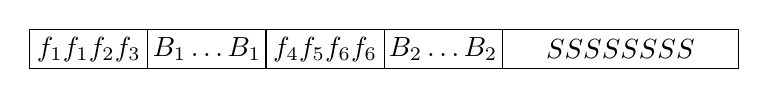
\begin{tikzpicture}[scale=1]
\draw (0,0.0) +(-.75,-.25) rectangle ++(.75,.25);
\visible<3->
{
\draw (0,0.0) node{$f_1 f_1 f_2 f_3$};
}
\draw (1.5,0) +(-.75,-.25) rectangle ++(.75,.25);
\visible<2->
{
\draw (1.5,0) node{$B_1 \hdots B_1$};
}
\draw (3,0) +(-.75,-.25) rectangle ++(.75,.25);
\visible<3->
{
\draw (3,0) node{$f_4 f_5 f_6 f_6$};
}
\draw (4.5,0) +(-.75,-.25) rectangle ++(.75,.25);
\visible<2->
{
\draw (4.5,0) node{$B_2 \hdots B_2$};
}
\draw (6.75,0) +(-1.5,-.25) rectangle ++(1.5,.25);
\visible<4->
{
\draw (6.75,0)node{$SSSSSSSS$};
}
\end{tikzpicture}
\end{figure}

\end{frame}

\begin{frame}{Greedy Algorithm}

We showed that, for a plane filled with couples, the simplest sweep algorithm is optimal due to the following observation:

\begin{figure}[H]
\centering
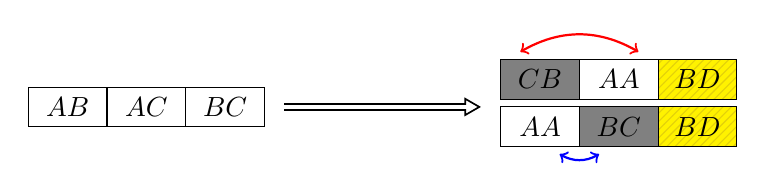
\begin{tikzpicture}[scale=1]
\draw (-6.0,0.25) +(-.5,-.25) rectangle ++(.5,.25);
\draw (-6.0,0.25) node{$A B$};x
\draw (-5.0,0.25) +(-.5,-.25) rectangle ++(.5,.25);
\draw (-5.0,0.25) node{$A C$};
\draw (-4.0,0.25) +(-.5,-.25) rectangle ++(.5,.25);
\draw (-4.0,0.25) node{$B C$};

\draw[vecArrow] (-3.25,0.25) to (-0.75,0.25);

\visible<2>
{
      \draw [thick,red,bend left,<->] (-0.25,0.95) to (1.25,0.95);
}

\visible<4->
    {
      \fillGray (0.0,.60) +(-.5,-.25) rectangle ++(.5,.25);
      \fillGray (1.0,0) +(-.5,-.25) rectangle ++(.5,.25);

      \fillYellow (2.0,.60) +(-.5,-.25) rectangle ++(.5,.25);
      \fillYellow (2.0,0) +(-.5,-.25) rectangle ++(.5,.25);

    }

\visible<2->
    {
       \draw (0.0,.60) +(-.5,-.25) rectangle ++(.5,.25);
       \draw (0.0,.60) node{$C B$};
       \draw (1.0,.60) +(-.5,-.25) rectangle ++(.5,.25);
       \draw (1.0,.60) node{$A A$};
       \draw (2.0,.60) +(-.5,-.25) rectangle ++(.5,.25);
       \draw (2.0,.60) node{$B D$};
    }
\visible<3>
{
      \draw [thick,blue,bend right,<->]  (0.25,-0.35) to (0.75,-0.35);
}
\visible<3->
    {
      \draw (0,0.0) +(-.5,-.25) rectangle ++(.5,.25);
      \draw (0,0.0) node{$A A$};
      \draw (1.0,0) +(-.5,-.25) rectangle ++(.5,.25);
      \draw (1.0,0) node{$B C$};
      \draw (2.0,0) +(-.5,-.25) rectangle ++(.5,.25);
      \draw (2.0,0) node{$B D$};
    }
\end{tikzpicture}
\end{figure}

\only<2>
{
The {\color{red}{red} exchange.}
}

\only<3>
{
And the {\color{blue}{blue} exchange.}
}

\only<4>
{
Leave the remaining passengers' seating locations equivalent.
}


\end{frame}

\begin{frame}\frametitle{Mixed Couples and Singles: Alignment}

With singletons and couples both present, we have to deal with alignment issues.

\begin{figure}[H]
\centering
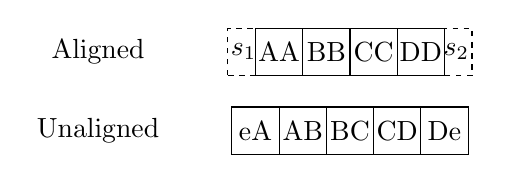
\begin{tikzpicture}[scale=1]
\draw (-2,1) node{Aligned};
\draw[dash pattern= on 2pt off 2pt] (-0.15,1) +(-.2,-.3) rectangle ++(.15,.3);
\draw (-0.15,1) node{$s_1$};
\draw (0.3,1) +(-.3,-.3) rectangle ++(.3,.3);
\draw (0.3,1) node{AA};
\draw (0.9,1) +(-.3,-.3) rectangle ++(.3,.3);
\draw (0.9,1) node{BB};
\draw (1.5,1) +(-.3,-.3) rectangle ++(.3,.3);
\draw (1.5,1) node{CC};
\draw (2.1,1) +(-.3,-.3) rectangle ++(.3,.3);
\draw (2.1,1) node{DD};
\draw[dash pattern= on 2pt off 2pt] (2.55,1) +(-.15,-.3) rectangle ++(.2,.3);
\draw (2.55,1) node{$s_2$};

\draw (-2,0) node{Unaligned};
\draw (0.0,0) +(-.3,-.3) rectangle ++(.3,.3);
\draw (0.0,0) node{eA};
\draw (0.6,0) +(-.3,-.3) rectangle ++(.3,.3);
\draw (0.6,0) node{AB};
\draw (1.2,0) +(-.3,-.3) rectangle ++(.3,.3);
\draw (1.2,0) node{BC};
\draw (1.8,0) +(-.3,-.3) rectangle ++(.3,.3);
\draw (1.8,0) node{CD};
\draw (2.4,0) +(-.3,-.3) rectangle ++(.3,.3);
\draw (2.4,0) node{De};
\end{tikzpicture}
\end{figure}

Aligned sets of matched couples are called {\it blocks}.  They have even numbers of seats.

\end{frame}

\begin{frame}[t]{Dynamic Program for Alignment}

Odd length gaps of singletons and unpaired couples are labeled $O_i$ and shown inside circles.

Complexes of blocks and even gaps, starting and ending with a block, have the form $B_1EB_2E...B_k$.  The associated number of required swaps, $N_i$ is  $\sum_{j=1}^k B_j$.  They are labeled $E_i$ and shown in squares. 

\begin{figure}[H]
\centering
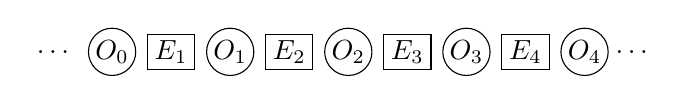
\begin{tikzpicture}[scale=.75]
\draw (0.5,0) node{$\hdots$};

\draw (1.8,.3) +(-.3,-.3) circle (.4);
\draw (1.5,0) node{$O_0$};

\foreach \x in {1, 2, 3, 4}
{
  \draw (0.5+2*\x,0) +(-.4,-.3) rectangle ++(.4,.3);
  \draw (0.5+2*\x,0) node{$E_\x$};
  \draw (2*\x+1.8,.3) +(-.3,-.3) circle (.4);
  \draw (2*\x+1.5,0) node{$O_\x$};
}
\draw (10.3,0) node{$\hdots$};
\end{tikzpicture}
\end{figure}

The number of swaps required by even complex $x$ to have closed $k$ odd gaps, $S(x,k)$ follows the recurrence:

\begin{equation*}
  S(x,k) = \min S(x-2, k-2) + N_x, S(x-1,k)
\end{equation*}

\end{frame}

\begin{frame}[fragile]
\frametitle{Non-Optimality}

\begin{columns}
\begin{column}{.5\textwidth}
Non-local win-win situations tie the alignment of two pairs of passengers to a possible saving of one swap.

\begin{figure}[H]
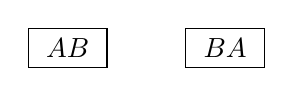
\begin{tikzpicture}[scale=1]
\draw (0,0.0) +(-.5,-.25) rectangle ++(.5,.25);
\draw (0,0.0) node{$A B$};x
\draw (2.0,0) +(-.5,-.25) rectangle ++(.5,.25);
\draw (2.0,0) node{$B A$};
\end{tikzpicture}
\end{figure}
\end{column}
\begin{column}{.5\textwidth}
\begin{figure}[H]

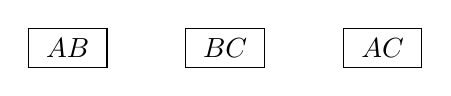
\begin{tikzpicture}[scale=1]
\draw (0,0.0) +(-.5,-.25) rectangle ++(.5,.25);
\draw (0,0.0) node{$A B$};x
\draw (2.0,0) +(-.5,-.25) rectangle ++(.5,.25);
\draw (2.0,0) node{$B C$};
\draw (4.0,0) +(-.5,-.25) rectangle ++(.5,.25);
\draw (4.0,0) node{$A C$};
\end{tikzpicture}
\end{figure}

Win-win 2-chains can be generalized to any length non-local k-chains.

\end{column}
\end{columns}

\begin{block}{Performance Factor}
Any algorithm that ignores $k$-chains may require up to $\frac{k}{k-1}$ times the optimal number of swaps.  Since we ignore 2-chains, our algorithm is only a 2 factor approximation.
\end{block}

\end{frame}

\section[DNA]{Genetic Intervals}
\begin{frame}[t]{DNA Copy Analysis}
  \begin{figure}[H] 
    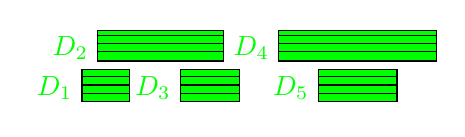
\begin{tikzpicture}[scale=1]

      % We want 5 rectangles that look like:
      %     2222222222       4444444444444444
      % 1111111   33333333       55555555
      \draw (0,0) rectangle (.6,.4);
      \fillGreen (0,0) rectangle (.6,.4);
      \node[green] at (0,-.1) [above left] {$D_1$};

      \draw (.2,.5) rectangle (1.8,.9);
      \fillGreen (.2,.5) rectangle (1.8,.9);
      \node[green] at (.2,.4) [above left] {$D_2$};

      \draw (1.25,0) rectangle (2,.4);
      \fillGreen (1.25,0) rectangle (2,.4);
      \node[green] at (1.25,-.1) [above left] {$D_3$};

      \draw (2.5,.5) rectangle (4.5,.9);
      \fillGreen (2.5,.5) rectangle (4.5,.9);
      \node[green] at (2.5,.4) [above left] {$D_4$};

      \draw (3,0) rectangle (4,.4);
      \fillGreen (3,0) rectangle (4,.4);
      \node[green] at (3,-.1) [above left] {$D_5$};

    \end{tikzpicture} 
    \caption{Simple 5 defect example}
  \end{figure}

  \begin{itemize}
  \item Cancer patients' genomes are 1D objects, i.e. lines.
  \item Closed intervals along that line have genetic abnormalities, and are labeled ``defects.''
  \item Goal: Across a number of patients, identify the $k$ most promising common regions.
  \end{itemize}


\end{frame}

\begin{frame}[t]{Explaining / Scoring}
  \begin{figure}[H] 
    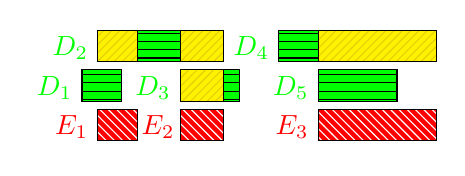
\begin{tikzpicture}[scale=1]

      % We want 5 rectangles that look like:
      %     2222222222       4444444444444444
      % 1111111   33333333       55555555
      \draw (0,0) rectangle (.5,.4);
      \fillGreen (0,0) rectangle (.5,.4);
      \node[green] at (0,-.1) [above left] {$D_1$};

      \draw (.2,.5) rectangle (1.8,.9);
      \fillGreen (.2,.5) rectangle (1.8,.9);
      \node[green] at (.2,.4) [above left] {$D_2$};

      \draw (1.25,0) rectangle (2,.4);
      \fillGreen (1.25,0) rectangle (2,.4);
      \node[green] at (1.25,-.1) [above left] {$D_3$};

      \draw (2.5,.5) rectangle (4.5,.9);
      \fillGreen (2.5,.5) rectangle (4.5,.9);
      \node[green] at (2.5,.4) [above left] {$D_4$};

      \draw (3,0) rectangle (4,.4);
      \fillGreen (3,0) rectangle (4,.4);
      \node[green] at (3,-.1) [above left] {$D_5$};

      %Now draw some explanations

      %% Extends past D_1, scoring only on D_2
      \draw (.2,-.5) rectangle (.7,-.1);
      \fillRed (.2,-.5) rectangle (.7,-.1);
      \node[red] at (.2,-.6) [above left] {$E_1$};

      \fillYellow (.2,.5) rectangle (.7,.9);

      % Overlape D_2 and D_3
      \draw (1.25,-.5) rectangle (1.8,-.1);
      \fillRed (1.25,-.5) rectangle (1.8,-.1);
      \node[red] at (1.3,-.6) [above left] {$E_2$};

      \fillYellow (1.25,.5) rectangle (1.8,.9);
      \fillYellow (1.25,0) rectangle (1.8,.4);
      %% Extends past D_5, scoring only on D_4
      \draw (3,-.5) rectangle (4.5,-.1);
      \fillRed (3,-.5) rectangle (4.5,-.1);
      \node[red] at (3,-.6) [above left] {$E_3$};

      \fillYellow (3,.5) rectangle (4.5,.9);

    \end{tikzpicture}
  \end{figure}

  \only<1>{
    Given a set $D$ of defects, find a set $E$ of $k$ closed intervals, or \textit{explanations}, maximizing:

    \begin{equation*}
      \sum_{D_j \in D}  \Big|\bigcup_{(E_i \in E) \cap (E_i \subseteq D_j)} E_i \Big| \frac{1}{|D_j|}
    \end{equation*}
  }

  \only<2->{
    \begin{itemize}
    \item An explanation explains a defect iff it is a subset of that defect.
    \item A specific region of a defect can only be explained once.
    \item An explanation can explain portions of multiple defects.
    \item A defect can be explained by multiple explanations.
    \item Maximum score per defect is 1.
    \end{itemize}
  }

\end{frame}

\begin{frame}{Maximal Explanations}

  \only<1>{
    How many explanations do we have to consider when finding the optimal set?  
  }

  \only<2>{
    The explanation $E_1$ only explains $D_1$, but better scoring explanations exist which also explain $D_1$.
  }

  \only<3>{
    The new explanation $E_2$ is formed by moving the left endpoint of $E_1$ until it matches the left endpoint of $D_1$.
  }

  \only<4>{
    We further improve $E_3$ to become a maximal explanation by making its right endpoint match the right endpoint of $D_1$.
  }

  \only<5>{
    The explanation $E_4$ is trivially non-maximal: it does not explain any defect at all.
  }

  \only<6>{
    $E_5$ is also maximal: its left endpoint is the left endpoint of $D_3$ and its right endpoint matches $D_6$.
  }

  \only<7>{
    Maximal explanations start and end at defect endpoints.  There are $O(n^2)$ maximal explanations for any defect set.
  }

  \begin{figure}[H]
    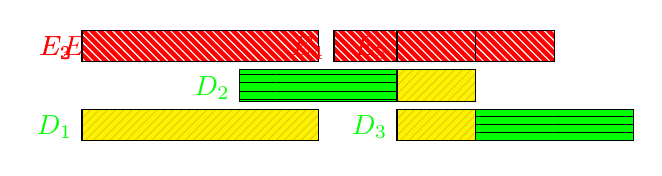
\begin{tikzpicture}[scale=1]

      \uncover<1-> {
        \draw (0,0) rectangle (3,.4);
        \fillGreen (0,0) rectangle (3,.4);
        \node[green] at (0,-.1) [above left] {$D_1$};

        \draw (2,.5) rectangle (5,.9);
        \fillGreen (2,.5) rectangle (5,.9);
        \node[green] at (2,.4) [above left] {$D_2$};

        \draw (4,0) rectangle (7,.4);
        \fillGreen (4,0) rectangle (7,.4);
        \node[green] at (4,-.1) [above left] {$D_3$};
      }

      \uncover<2> {

        \draw (.3,1) rectangle (2.3,1.4);
        \fillRed (0.3,1) rectangle (2.3,1.4);
        \node[red] at (0.3,.9) [above left] {$E_1$};

        \fillYellow (.3,0) rectangle (2.3,.4);
      }

      \uncover<3>  {

        \draw (0,1) rectangle (2.3,1.4);
        \fillRed (0,1) rectangle (2.3,1.4);
        \node[red] at (0,.9) [above left] {$E_2$};

        \fillYellow (0,0) rectangle (2.3,.4);
      }

      \uncover<4,7-> {

        \draw (0,1) rectangle (3,1.4);
        \fillRed (0,1) rectangle (3,1.4);
        \node[red] at (0,.9) [above left] {$E_3$};

        \fillYellow (0,0) rectangle (3,.4);
      }

      \uncover<5> {

        \draw (3.2,1) rectangle (6,1.4);
        \fillRed (3.2,1) rectangle (6,1.4);
        \node[red] at (3.2,.9) [above left] {$E_4$};
      }

      \uncover<6-> {

        \draw (4,1) rectangle (5,1.4);
        \fillRed (4,1) rectangle (5,1.4);
        \node[red] at (4,.9) [above left] {$E_5$};

        \fillYellow (4,0) rectangle (5,.4);
        \fillYellow (4,.5) rectangle (5,.9);
      }

    \end{tikzpicture}
  \end{figure}

\end{frame}

\begin{frame}[t]{Greedy Algorithm: Illustration by Worst Case Example}

  \begin{figure}[H]
    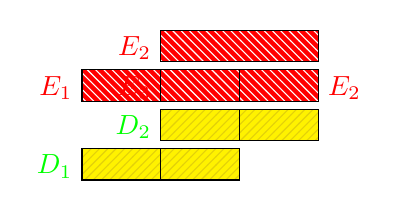
\begin{tikzpicture}[scale=1]

      % We want
      %     2222222222
      % 1111111


      \uncover<1->{
        \draw (0,0) rectangle (2,.4);
        \fillGreen (0,0) rectangle (2,.4);
        \node[green] at (0,-.1) [above left] {$D_1$};

        \draw (1,.5) rectangle (3,.9);
        \fillGreen (1,.5) rectangle (3,.9);
        \node[green] at (1,.4) [above left] {$D_2$};
      }

      \uncover<2>{
        \draw (0,1) rectangle (2,1.4);
        \fillRed (0,1) rectangle (2,1.4);
        \node[red] at (0,.9) [above left] {$E_1$};


        \draw (1,1.5) rectangle (3,1.9);
        \fillRed (1,1.5) rectangle (3,1.9);
        \node[red] at (1,1.4) [above left] {$E_2$};

        \fillYellow (0,0) rectangle (2,.4);
        \fillYellow (1,.5) rectangle (3,.9);  
      }

      \uncover<3->{
        \draw (1,1) rectangle (2,1.4);
        \fillRed (1,1) rectangle (2,1.4);
        \node[red] at (1,.9) [above left] {$E_3$};

        \fillYellow (1,0) rectangle (2,.4);
        \fillYellow (1,.5) rectangle (2,.9);
        
      }

      \uncover<4->{
        \draw (2,1) rectangle (3,1.4);
        \fillRed (2,1) rectangle (3,1.4);
        \node[red] at (3,.9) [above right] {$E_2$};

        \fillYellow (2,.5) rectangle (3,.9);
        
      }
    \end{tikzpicture} 
  \end{figure}

  This is the simplest example where Greedy is non-optimal:

  \only<2>{
    When we allow 2 explanations to cover 2 defects, the obvious correct answer is $E_1 = D_1$ and $E_2 = D_2$.
  }

  \only<3->{
    In the first step of greedy, we select the high scoring center region.
  }

  \only<4->{
    This leaves us with lower scoring side regions for our next selection.  Greedy only scored $\frac34$ of the maximum attainable score by making a bad first selection.
  }
\end{frame}

\begin{frame}[t]{1-OPT Exchange Algorithm}

  \begin{figure}[H]
    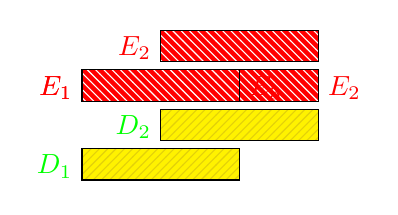
\begin{tikzpicture}[scale=1]

      % We want
      %     2222222222
      % 1111111


      \draw (0,0) rectangle (2,.4);
      \fillGreen (0,0) rectangle (2,.4);
      \node[green] at (0,-.1) [above left] {$D_1$};

      \draw (1,.5) rectangle (3,.9);
      \fillGreen (1,.5) rectangle (3,.9);
      \node[green] at (1,.4) [above left] {$D_2$};

      \uncover<1,2,3>{
        \draw (1,1) rectangle (2,1.4);
        \fillRed (1,1) rectangle (2,1.4);

        \fillYellow (1,0) rectangle (2,.4);
        \fillYellow (1,.5) rectangle (2,.9);
      }

      \uncover<1,2>  {
        \node[red] at (1,.9) [above left] {$E_3$};
      }
      
      \uncover<1>  {
        \draw (2,1) rectangle (3,1.4);
        \fillRed (2,1) rectangle (3,1.4);
        \node[red] at (3,.9) [above right] {$E_2$};

        \fillYellow (2,.5) rectangle (3,.9);
        
      }

      \uncover<3>{
        % Fix label covered in step 3 by $E_1$
        \node[red] at (2,.9) [above right] {$E_3$};
      }

      \uncover<3,4> {
        \draw (0,1) rectangle (2,1.4);
        \fillRed (0,1) rectangle (2,1.4);
        \node[red] at (0,.9) [above left] {$E_1$};
        \fillYellow (0,0) rectangle (2,.4);

      }

      \uncover<5->{
        \draw (0,1) rectangle (2,1.4);
        \fillRed (0,1) rectangle (2,1.4);
        \node[red] at (0,.9) [above left] {$E_1$};


        \draw (1,1.5) rectangle (3,1.9);
        \fillRed (1,1.5) rectangle (3,1.9);
        \node[red] at (1,1.4) [above left] {$E_2$};

        \fillYellow (0,0) rectangle (2,.4);
        \fillYellow (1,.5) rectangle (3,.9);  
      }
    \end{tikzpicture} 
  \end{figure}

  \only<1>{
    A 1-OPT refinement solves the $n=k=2$ worst case defect set.  It starts with the greedy solution.
  }

  \only<2,3>{
    It then removes each explanation in turn ($E_2$ in this case) and tries to replace it with an explanation that scores at least as much.
  }

  \only<3>{
    Here $E_1$ was selected to replace $E_2$.
  }

  \only<4,5> {
    Now we remove $E_3$ to try and improve the score.
  }

  \only<5> {
    The best scoring maximal explanation remaining is $E_2$.
  }

  \only<6> {
    We test to see if removing an explanation and replacing it can further improve the score.  Since it cannot, the algorithm terminates.
  }

\end{frame}

\begin{frame}[t]{Unfortunately, 1-OPT Isn't Optimal}

  \begin{figure}[H]
    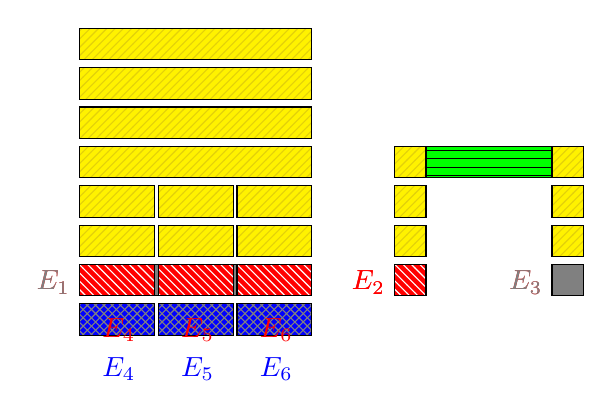
\begin{tikzpicture}[scale=1]

      % 6 small rectangles on the left in 2 rows of 3
      \foreach \x in {0,1,2} {
        \foreach \y in {0,1} {
          \draw (0+\x,0+\y/2) rectangle (.95+\x,.4+\y/2);
          \fillGreen (0+\x,0+\y/2) rectangle (.95+\x,.4+\y/2);
        }
      }
      
      % 4 Wide caps on those small rectangles
      \foreach \y in {0,1,2,3} {
        \draw (0,1+\y/2) rectangle (2.95,1.4+\y/2);
        \fillGreen (0,1+\y/2) rectangle (2.95,1.4+\y/2);
      }

      
      \foreach \y in {0,1} {
        \foreach \x in {4, 6} {
          \draw (0+\x,0+\y/2) rectangle (.4+\x,.4+\y/2);
          \fillGreen (0+\x,0+\y/2) rectangle (.4+\x,.4+\y/2);
        }
      }                  
      \draw (4,1) rectangle (6.4,1.4);
      \fillGreen (4,1) rectangle (6.4,1.4);

      \uncover<2,4,6>{
        \fillRed (0,-.5) rectangle (2.95, -.1);
        \node[red] at (0,-.6) [above left] {$E_1$};
        \foreach \y in {0,1,2,3} {
          \fillYellow (0,1+\y/2) rectangle (2.95,1.4+\y/2);
        }
      } %uncover<2.4>

      \uncover<2,4,5>{
        \draw (4,-.5) rectangle (4.4, -.1);
        \fillRed (4,-.5) rectangle (4.4, -.1);
        \node[red] at (4,-.6) [above left] {$E_2$};
        
        \draw (6,-.5) rectangle (6.4, -.1);
        \fillRed (6,-.5) rectangle (6.4, -.1);
        \node[red] at (6,-.6) [above left] {$E_3$};

        
        \foreach \y in {0,1,2} {
          \foreach \x in {4, 6} {
            \fillYellow (0+\x,0+\y/2) rectangle (.4+\x,.4+\y/2);
          }
        }                                               
      } % uncover<2,4,5>


      \uncover<5,6>{


        \foreach \x in {4,5,6} {
          \fillBlue (-4+\x,-1.0) rectangle (-3.05+\x,-.6);
          \node[blue] at (-3.5+\x,-1.7) [above] {$E_\x$};
        }

      }

      \uncover<5>{

        \fillGray (0,-.5) rectangle (2.95, -.1);
        \node[gray] at (0,-.6) [above left] {$E_1$};
      }

      \uncover<6>{
        \foreach \y in {0,1,2} {
          \fillYellow (4,0+\y/2) rectangle (4.4,.4+\y/2);
        }
        \fillRed (4,-.5) rectangle (4.4, -.1);
        \node[red] at (4,-.6) [above left] {$E_2$};

        \fillGray (6,-.5) rectangle (6.4, -.1);
        \node[gray] at (6,-.6) [above left] {$E_3$};

      }

      \uncover<3,7>{
        \foreach \x in {4,5,6} {
          \fillRed (-4+\x,-.5) rectangle (-3.05+\x,-.1);
          \node[red] at (-3.5+\x,-1.2) [above] {$E_\x$};
        }

        \foreach \x in {0,1,2} {
          \foreach \y in {0,1} {
            \fillYellow (0+\x,0+\y/2) rectangle (.95+\x,.4+\y/2);
          }
        }
        \foreach \y in {0,1,2,3} {
          \fillYellow (0,1+\y/2) rectangle (2.95,1.4+\y/2);
        }
      } % uncover 3
      
    \end{tikzpicture}
  \end{figure}          

  \only<1>{  
    1-OPT fails to optimally explain these 15 defects with 3 explanations. 
  }

  \only<2>{
    This is a non-optimal solution.

    $E_1$ scores 4.

    Both $E_2$ and $E_3$ score $2+\epsilon$.

    They total $8 + 2\epsilon$.
  }

  \only<3>{
    This is the optimal solution.

    Each of $E_4, E_5$ and $E_6$ score $3 \frac13$.

    This total of $10$ beats our bad solution.
  }

  \only<4,5,6>{
    There is no 1-OPT path from this bad case to OPT.
  }

  \only<5>{
    Without $E_1$ in place, $E_4, E_5$ and $E_6$ only score $3 \frac13$, which is lower than $E_1$'s score of 4.
  }

  \only<6>{
    When $E_3$ is offered for exchange, $E_4, E_5$ and $E_6$ only score $2$ which is less than the $2+\epsilon$ that $E_3$ had scored.
  }

  \only<7>{
    Since this optimal arrangement cannot be reached from the starting point we chose, 1-OPT is not guaranteed to be optimal for $n>k$.
  }

\end{frame}

\begin{frame}[t]{Dynamic Programming PTAS}

\only<1>{

In order to solve this with a {\it fixed depth} dynamic program, we need discrete states and a separation between active and inactive regions.

}

\begin{figure}[ht!] \centering
\begin{tikzpicture}[xscale=1,yscale=.5]

\coordinate (L1) at (1,0.0);
\coordinate (R1) at (7,0.8);

\coordinate (L2) at (2,1.0);
\coordinate (R2) at (8,1.8);

\coordinate (L3) at (4,2.0);
\coordinate (R3) at (9,2.8);

\coordinate (L4) at ( 6,3.0);
\coordinate (R4) at (10,3.8);

\coordinate (L5) at (3,3.0);
\coordinate (R5) at (5,3.8);

\coordinate (SL1) at (1,-1.0);
\coordinate (SR1) at (2,-0.2);

\coordinate (SL2) at (2,-2.0);
\coordinate (SR2) at (4,-1.2);

\coordinate (SL2) at (2,-2.0);

\coordinate (inactiveLabel) at (2,-2.0);

\coordinate (SL3) at (3,-1.0);
\coordinate (SR3) at (5,-0.2);

\coordinate (SL4) at (4,-2.0);
\coordinate (SR4) at (5,-1.2);
\coordinate (SR4-6) at (6,-1.2);
\coordinate (SR4-7) at (7,-1.2);

\coordinate (setLabel) at (6,-2);
\coordinate (activeLabel) at (6,-3);

\coordinate (depthBottom) at (7.1,-0.25);
\coordinate (depthTop)    at (7.1,-2);

\coordinate (SL5) at (6,-1.0);
\coordinate (SR5) at (7,-0.2);

\coordinate (futureLabel) at (9,-2);

\foreach \rect in {1,2,3,4,5} {
  \draw (L\rect) rectangle (R\rect);
  \fillGreen (L\rect) rectangle (R\rect);
}

\only<1>{
  \fillYellow (SL1) rectangle (SR1);
  \fillYellow (SL2) rectangle (SR2);
  \fillYellow (SL3) rectangle (SR3);

  \fillRed    (SL4) rectangle (SR4-7);
  \fillRed    (SL5) rectangle (SR5);

  \node[citrine] at (inactiveLabel) [below] {Placed Explanations}; 
  \node[black] at (activeLabel) [below] {Active Zone};
  \node[red] at (setLabel) [below] {Active Set};
  \node[blue] at (futureLabel) [below] {Future Explanations};

  \draw[decorate,decoration={brace,amplitude=6pt}] (depthBottom) -- (depthTop) node [black,midway,xshift=56pt] {2 {\color{red} Active}, Depth $\geq$ 2};


  \draw (5,-2.0) -- (5,4.3);
  \draw (7,-2.0) -- (7,4.3);

}

\only<2->{

  \fillYellow (SL1) rectangle (SR1);
  \fillYellow (SL2) rectangle (SR2);

}

\only<2-3>{

  \fillRed    (SL3) rectangle (SR3);

  \draw (3,-2.0) -- (3,4.3);
  \node[black] at (3,-2.0) [below] {$a$};

  \draw (5,-2.0) -- (5,4.3);
  \node[black] at (5,-2.0) [below] {$b$};


}

\only<3>{
  \fillRed    (SL4) rectangle (SR4);
}

\only<4>{
  \fillRed    (SL3) rectangle (SR3);
  \fillRed    (SL4) rectangle (SR4);

  \draw (5,-2.0) -- (5,4.3);
  \node[black] at (5,-2.0) [below] {$a$};

  \draw (4,-2.0) -- (4,4.3);
  \node[black] at (4,-2.0) [below] {$a-1$};
}

\only<5-7,9>{
  \fillYellow (SL3) rectangle (SR3);
  \fillRed    (SL4) rectangle (SR4-7);
}

\only<8>{
  \fillYellow (SL3) rectangle (SR3);
  \fillRed    (SL4) rectangle (SR4-6);
}

\only<5,7,9>{
  \draw (5,-2.0) -- (5,4.3);
  \node[black] at (5,-2.0) [below] {$a$};

  \draw (7,-2.0) -- (7,4.3);
  \node[black] at (7,-2.0) [below] {$b$};
}

\only<6>{
  \draw (4,-2.0) -- (4,4.3);
  \node[black] at (4,-2.0) [below] {$a-1$};

  \draw (7,-2.0) -- (7,4.3);
  \node[black] at (7,-2.0) [below] {$b$};
}

\only<8>{
  \draw (5,-2.0) -- (5,4.3);
  \node[black] at (5,-2.0) [below] {$a$};

  \draw (6,-2.0) -- (6,4.3);
  \node[black] at (6,-2.0) [below] {$b-1$};
}


\end{tikzpicture} 
\end{figure}

\only<1>{



}

\only<2-3>{
Transformation 1 is starting a new active explanation:

\begin{center}
\begin{tabular}{l|ll}
 & Old & New \\ \hline
Num Placed & k-1 & \only<3>{k} \\
Left & a         & \only<3>{a} \\
Right & b        & \only<3>{b} \\
Active Set & S-e & \only<3>{S} \\
\end{tabular}
\end{center}
}

\only<4-5>{
Transformation 2 is ending an active explanation:

\begin{center}
\begin{tabular}{l|ll}
 & Old & New \\ \hline
Num Placed & k       & \only<5>{k} \\
Left       & a-1     & \only<5>{a} \\
Right      & a       & \only<5>{b} \\
Active Set & S+(x,a) & \only<5>{S} \\
\end{tabular}
\end{center}
}

\only<6-7>{
Transformation 3 is shrinking the active zone:

\begin{center}
\begin{tabular}{l|ll}
 & Old & New \\ \hline
Num Placed & k & \only<7>{k} \\
Left & a-1     & \only<7>{a} \\
Right & b      & \only<7>{b} \\
Active Set & S & \only<7>{S} \\
\end{tabular}
\end{center}
}

\only<8-9>{
Transformation 4 is expanding the active zone:

\begin{center}
\begin{tabular}{l|ll}
 & Old & New \\ \hline
Num Placed & k & \only<9>{k} \\
Left  & a      & \only<9>{a} \\
Right & b-1    & \only<9>{b} \\
Active Set & S & \only<9>{S} \\
\end{tabular}
\end{center}
}
\end{frame}

\begin{frame}[t]{Defect Primitives}
  Our LP formulation uses defect primitives: the portions of a defect between 2 adjacent starting/ending points.

  \begin{figure}[H]
    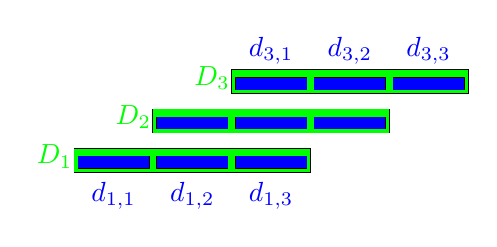
\begin{tikzpicture}[scale=1]

      \foreach \y in {1,2,3} {
        \draw (\y+1, \y/2) rectangle (\y+4, \y/2+.3);
        \fill[green] (\y+1, \y/2) rectangle (\y+4, \y/2+.3);
        \foreach \x in {1,2,3} {
          \draw (\x+\y+.05,\y/2 +.05) rectangle (\x+\y+.95,\y/2+.2);
          \fill[blue] (\x+\y+.05,\y/2 +.05) rectangle (\x+\y+.95,\y/2+.2);
        }
      }

      \foreach \x in {1,2,3} {
        \node[blue] at (1.5+\x,.5) [below] {$d_{1,\x}$};
      }
      
      \foreach \x in {1,2,3} {
        \node[blue] at (3.5+\x,1.75) [above] {$d_{3,\x}$};
      }
      
      
      \foreach \x in {1,2,3} {
        \node[green] at (\x+.75,.2+\x/2) {$D_\x$};
      }

    \end{tikzpicture} 
  \end{figure}

  Since both defect primitives and maximal explanations start and end at defect endpoints, an explantion will never explain fractional defect primitives.
\end{frame}

\begin{frame}[t]{LP Relaxation}

    \only<1>{Maximize the weighted sum of defect primitives explained.} 
    \only<2->{
      Maximize:
      \begin{equation*}
        \sum_i \sum_j p_{i,j} \frac{|d_{i,j}|}{|D_i|}
      \end{equation*}
    } 

    Subject to:

    \only<1-2>{ Each defect primitive is only explained if an $E_i$ that can explain it is in the solution set {\bf $E$}.} 
    \only<3->{\begin{equation*}
        \forall_{i,j} p_{i,j} \leq \sum_k e_k \cdot \Theta(E_k \subseteq D_i \wedge d_{i,j} \subseteq E_K )
    \end{equation*}
    }  

    \only<1-3>{We use at most $k$ explanations.}

    \only<4->{\begin{equation*}
        \sum_i e_i \leq k
      \end{equation*}
    }

    \only<1-4>{Primitives can only be counted once for score.

  $e_i$:    1 if explanation $E_i$ is in our explanation set, and 0 if not.

  $p_{i,j}$: 1 if defect primitive $d_{i,j}$, a part of defect $D_i$, is explained, 0 if it is not.
}

    \only<5->{\begin{eqnarray*}
        \forall_{i,j} p_{i,j} \in \{0, 1 \} \\
        \forall_{i,j} e_i \in \{0, 1 \} 
      \end{eqnarray*}
    }


\end{frame}

\begin{frame}[fragile]
\frametitle{Experimental Summary}

\begin{columns}
\begin{column}{0.5\textwidth}
\begin{figure}[ht!] \centering
  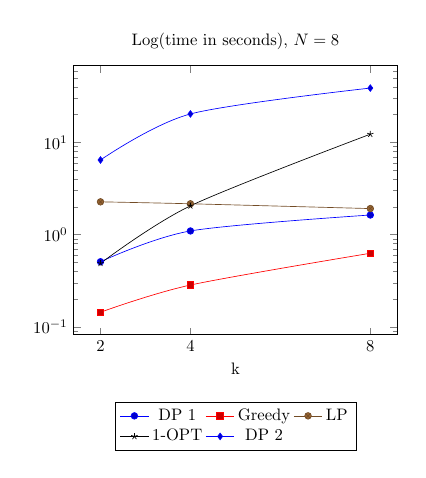
\begin{tikzpicture}[scale=0.6]
    \begin{axis}[ title={Log(time in seconds), $N=8$}, 
        xlabel=k,
        ymode=log,
        /pgfplots/xtick={2,4,8},
        legend style={at={(.5,-.25)},anchor=north,legend columns=3},
      ]
      \addplot+[smooth] coordinates {(2, 0.508) (4, 1.096) (8, 1.632) };    
      \addplot+[smooth] coordinates {(2, 0.144) (4, 0.284) (8, 0.628) };    
      \addplot+[smooth] coordinates {(2, 2.268) (4, 2.160) (8, 1.916) };    
      \addplot+[smooth] coordinates {(2, 0.488) (4, 2.052) (8,12.280) };    
      \addplot+[smooth] coordinates {(2, 6.448) (4,20.364) (8,38.868) };    
      \legend {DP 1, Greedy,  LP, 1-OPT, DP 2}
    \end{axis}
  \end{tikzpicture}
  \caption{Time to place $k$ explanations to cover 8 defects.}
\end{figure}
\end{column}
\begin{column}{0.5\textwidth}
\begin{figure}[ht!] \centering
  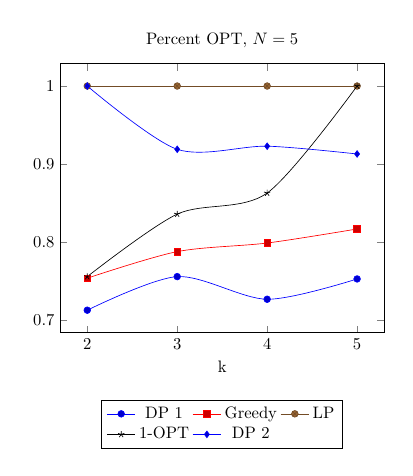
\begin{tikzpicture}[scale=.6]
    \begin{axis}[ title={Percent OPT, $N=5$}, 
        xlabel=k,
        /pgfplots/xtick={2,...,5},
        legend style={at={(.5,-.25)},anchor=north,legend columns=3},
      ]
      \addplot+[smooth] coordinates {(2, 0.713) (3, 0.756) (4, 0.727) (5,0.753)};    
      \addplot+[smooth] coordinates {(2, 0.754) (3, 0.788) (4, 0.799) (5,0.817)};    
      \addplot+[smooth] coordinates {(2, 1.00 ) (3, 1.00 ) (4, 1.00 ) (5, 1.00 )};    
      \addplot+[smooth] coordinates {(2, 0.756) (3, 0.836) (4, 0.863) (5,1) };    
      \addplot+[smooth] coordinates {(2, 1.00 ) (3, 0.919) (4, 0.923) (5, 0.913)};    
      \legend {DP 1, Greedy,  LP, 1-OPT, DP 2}
    \end{axis}
  \end{tikzpicture}
  \caption{Results for placing $2-5$ explanations to cover $5$ defects.}
\end{figure}
\end{column}
\end{columns}

\end{frame}

\begin{frame}[t]{Conclusions}

\begin{itemize}
\item For any $N=k$ case, greedy is no better than a $\frac34$ approximation.

\item For all observed $N=k$ cases, 1-OPT finds the optimal solution.

\item 1-OPT is an easy to implement improvement ot greedy, but runs slowly.

\item For any $d\geq 5$, the d-depth DP PTAS is better than a $\frac34$ approximation.  It would also take centuries to solve any realistically sized problems.

\item Integer programming solves this problem in most cases, and has $\Theta(n^2)$ constraints and variables .
\end{itemize}

\end{frame}

\section[Waiter]{Waiter Problem}

\begin{frame}\frametitle{Problem Overview}

We're placing objects, one at a time, both to the {\color{red!60} right} and {\color{blue!60} left} of a final center of mass. We calculate the {\color{citrine} center of mass} at every step.

\begin{figure}[ht!] \centering
  \begin{tikzpicture}[scale=.4]

    \draw[latex-latex] (-12,0) -- (10,0) ; %edit here for the axis
    \foreach \x in  {-11,-5,-3,-1,0,2,4,6,8} % edit here for the vertical lines
             { 
               \draw[shift={(\x,0)},color=black] (0pt,-3pt) -- (0pt,5pt) node[above] {\x};               
             }

    \posNode at (2,3)   { \only<6->{5} };
    \posNode at (4,3)   { \only<5->{4} };
    \posNode at (6,3)   { \only<4->{3} };
    \posNode at (8,3)   { \only<3->{2} };

    \negNode at ( -1,3) { \only<9->{8} };
    \negNode at ( -3,3) { \only<8->{7} };
    \negNode at ( -5,3) { \only<7->{6} };
    \negNode at (-11,3) { \only<2->{1} };

    \uncover<2->{ \negStop{-11,-2}; }

    \uncover<2-3>{\posStop{0,-2}; }

    \uncover<4>{  \posStop{1,-2}; }
    \uncover<5>{  \posStop{1.75,-2}; }
    \uncover<6->{ \posStop{1.8,-2}; }

    \uncover<2>{ \com{-11  ,0}; }
    \uncover<3>{ \com{-1.5 ,0}; }
    \uncover<4>{ \com{1.00 ,0}; }
    \uncover<5>{ \com{1.75 ,0}; }
    \uncover<6>{ \com{1.80 ,0}; }
    \uncover<7>{ \com{0.66 ,0}; }
    \uncover<8>{ \com{0.14 ,0}; }
    \uncover<9>{ \com{0.00 ,0}; }

    \only<10>{}

  \end{tikzpicture}
\end{figure}

\uncover<4->{We seek to minimize the the quantity $R-L$, where the interval $[${\color{blue} L}, {\color{red} R}$]$ always contains the {\color{citrine} center of mass}.}

\uncover<10>{This was a poorly chosen order with $|R-L|=12.8$.  We'll do better later.}

\end{frame}

\begin{frame}[t]{Hardness}

We can reduce any instance of 3-partition to an airplane seating problem fairly easily.  Required gadgets:

$M \rightarrow \infty$ neutral masses {\color{gray} initially placed at 0}.

$3N$ positive masses, {\color{red!60} one to be placed at each $x_i$}.

$N$ negative masses, {\color{blue!60} to be placed at -1}.

\begin{figure}[ht!] \centering
  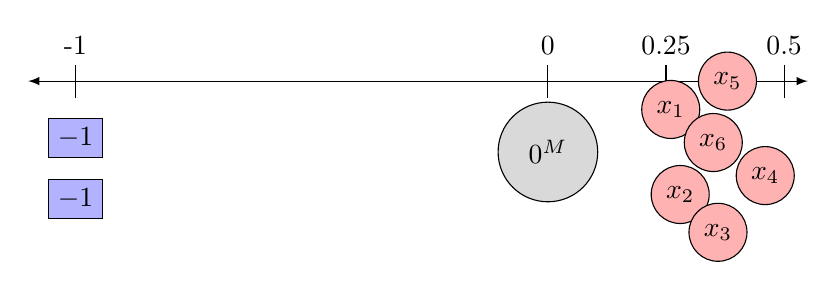
\begin{tikzpicture}[scale=6]


    \draw[latex-latex] (-1.1,0) -- (0.55,0) ; %edit here for the axis
    \foreach \x in  {-1,0,0.25,0.5} % edit here for the vertical lines
             { 
               \draw[shift={(\x,0)},color=black] (0pt,-1pt) -- (0pt,1pt) node[above] {\x};        
             };
             
     \draw[draw,fill=gray!30] (0,-.15) circle (3pt) node {$0^M$ };

     \posNode at (.26,-.06) {$x_1$};
     \posNode at (.28,-.24) {$x_2$};
     \posNode at (.36,-.32) {$x_3$};
     \posNode at (.46,-.20) {$x_4$};
     \posNode at (.38,-.00) {$x_5$};
     \posNode at (.35,-.13) {$x_6$};

     \negNode at (-1,-0.12) {$-1$};
     \negNode at (-1,-0.25) {$-1$};

\end{tikzpicture}
\end{figure}

If these masses can be placed while keeping the center of mass in $[\frac{-1}{M},0]$, then you have solved 3-partition.

\end{frame}

\begin{frame}[t]{Naive Bound on $|R-L|$}

Placing a mass $x_i$ in step $i$ gives you a running sum of $\Sigma_i$, and a center of mass of $c_i = \frac{\Sigma_i}{i}$. 

\begin{align*}
c_i - c_{i-1} &= \frac{\Sigma_i}{i} - \frac{\Sigma_{i-1}}{i-1} \\
|R-L| \geq c_i - c_{i-1} &= \frac{\Sigma_{i-1} + x_i}{i} - \frac{\Sigma_{i-1}}{i-1} \\
|R-L| &\geq  \frac{x_i}{i} - \frac{\Sigma_{i-1}}{i(i-1)} \geq  \frac{x_i}{i} \\
\end{align*}

Since adding $x_i$ moves the center of mass by, within a fudge factor, $\frac{|x_i|}{i}$, $|R-L|$ must be larger than this for all $i$.

Placing $x_i$ in order of sorted absolute value would minimize this quantity.

\end{frame}

\begin{frame}[t]{Simple Algorithm}

What if we always place the remaining mass closest to the origin?

\begin{figure}[ht!] \centering
  \begin{tikzpicture}[scale=.6]

    \draw[latex-latex] (-6,0) -- (6,0) ; %edit here for the axis
    \foreach \x in  {-5,0,1,2,3,4,5} % edit here for the vertical lines
             { 
               \draw[shift={(\x,0)},color=black] (0pt,-3pt) -- (0pt,5pt) node[above] {\x};               
             }

             
    \nullNode at (1,3)   { {\color{white} 1} };

    \posNode at (1,3)   { \only<2->{1} };
    \posNode at (2,3)   { \only<3->{2} };
    \posNode at (3,3)   { \only<4->{3} };
    \posNode at (4,3)   { \only<5->{4} };
    \posNode at (5,3)   { \only<6->{5} };

    \negNode at (-5,2) { \only<7->{6} };
    \negNode at (-5,3) { \only<8->{7} };
    \negNode at (-5,4) { \only<9->{8} };

    \uncover<2->{ \negStop{0,-2}; }

    \uncover<2>{  \posStop{1.00,-2}; }
    \uncover<3>{  \posStop{1.50,-2}; }
    \uncover<4>{  \posStop{2.00,-2}; }
    \uncover<5>{  \posStop{2.50,-2}; }
    \uncover<6->{ \posStop{3.00,-2}; }

    \uncover<2>{ \com{1.00 ,0}; }
    \uncover<3>{ \com{1.50 ,0}; }
    \uncover<4>{ \com{2.00 ,0}; }
    \uncover<5>{ \com{2.50 ,0}; }
    \uncover<6>{ \com{3.00 ,0}; }
    \uncover<7>{ \com{1.66 ,0}; }
    \uncover<8>{ \com{0.71 ,0}; }
    \uncover<9>{ \com{0.00 ,0}; }

  \end{tikzpicture}
\end{figure}

\uncover<9->{The center of mass is contained in the interval $[0,3]$. Our naive bound of $\frac{|x_i|}{i}$ gave us $|R-L| \geq 1$.

Unfortunately, this example scales and our bound underestimates even the optimum solution by a factor of $\sqrt{n}$. }

\end{frame}

\begin{frame}[t]{Tentpole Algorithm}

Sort the {\color{red!60} positive} and {\color{blue!60} negative} masses separately by absolute value.

Lowest absolute value number's list is active.  Place $|$lowest$|$ remaining on active list until the next would cause the running sum to be $|$greater$|$ than the $|$lowest$|$ inactive. Then switch lists.

\begin{figure}[ht!] \centering
  \begin{tikzpicture}[scale=.6]

    \draw[latex-latex] (-6,0) -- (6,0) ; %edit here for the axis
    \foreach \x in  {-5,0,1,2,3,4,5} % edit here for the vertical lines
             { 
               \draw[shift={(\x,0)},color=black] (0pt,-3pt) -- (0pt,5pt) node[above] {\x};               
             }

             
    \nullNode at (1,3)   { {\color{white} 1} };

    \posNode at (1,3)   { \only<2->{1} };
    \posNode at (2,3)   { \only<3->{2} };
    \posNode at (3,3)   { \only<5->{4} };
    \posNode at (4,3)   { \only<6->{5} };
    \posNode at (5,3)   { \only<8->{7} };

    \negNode at (-5,2) { \only<4->{3} };
    \negNode at (-5,3) { \only<7->{6} };
    \negNode at (-5,4) { \only<9->{8} };

    \uncover<2-3>{  \negStop{0,-2}; }
    \uncover<4->{ \negStop{-0.66,-2}; }

    \uncover<2>{  \posStop{1.00,-2}; }
    \uncover<3->{ \posStop{1.50,-2}; }

    \uncover<2>{ \com{1.00 ,0}; }
    \uncover<3>{ \com{1.50 ,0}; }
    \uncover<4>{ \com{-.66 ,0}; }
    \uncover<5>{ \com{0.25 ,0}; }
    \uncover<6>{ \com{1.00 ,0}; }
    \uncover<7>{ \com{0.00 ,0}; }
    \uncover<8>{ \com{0.71 ,0}; }
    \uncover<9>{ \com{0.00 ,0}; }

  \end{tikzpicture}
\end{figure}

\only<4>{
Because {\color{red!60}$1+2+3$} {\color{blue!60} $\geq 5$}, we switched lists after placing {\color{red!60}$2$}.
}

\only<5>{
Because {\color{blue!60}$|-2-5|$} {\color{red!60} $\geq 4$}, we switched lists after placing the first {\color{blue!60}$-5$}.
}

\only<7>{
Because {\color{red!60}$5+5$} {\color{blue!60} $\geq 5$}, we switched lists after placing {\color{red!60}$4$}.
}

\only<8>{
Because {\color{blue!60}$|0-5|$} {\color{red!60} $\geq 5$}, we switched lists after placing the second {\color{blue!60}$-5$}.
}

\only<9>{There are no {\color{red!60} positives} left, so place the remaining {\color{blue!60} negatives}.}

\end{frame}

\begin{frame}[t]{Tentpole Bound}

\begin{itemize}
\item The tentpole lower bound is: $|R-L|\geq \frac{|x_i|}{\pi_i}$.  $\pi_i$ is the placement order for the tentpole algorithm.  

\item Any number placed after switching lists potentially moves the CoM from  $R$ to $L$.  Such a tentpole number ``holds the interval open.''

\item This lower bound is never less than $\frac12$ the length of OPT. It is occasionally tight.

\item The tentpole algorithm is guaranteed to return an interval no worse than $2.7$ times this bound.
\end{itemize}

\end{frame}

\begin{frame}[t]{Staircase: The Best Sorted Heuristic}

Tentpole was a sorted heuristic: it placed positive and negative elements in order of increasing magnitude.  After placing {\color{red!60} $J$} positive elements and {\color{blue!60} $K$} negative elements, the center of mass is:

\begin{align*} 
C(J,K) = \frac{\sum_{j=1}^{J} p_j + \sum_{k=1}^{K} n_k }{J+K}
\end{align*}

This can be represented as a matrix with some nice properties.

\end{frame}

\begin{frame}[t]{Staircase By Example}


\only<1>{

\begin{align*}
P &= \{1,2,3,4,5\} \\
N &= \{-5,-5,-5\} \\
\end{align*}

With these positive and negative masses, we form the $C$ matrix:

\begin{table} \centering
\begin{tabular}{cccccc}
  0  &   1  &  1.5  &  2    & 2.5 & 3 \\
 -5  &  -2  & -0.66 & 0.25  &  1  & 1.66 \\
 -5  &  -3  & -1.75 & -0.8  &  0  &  0.71 \\
 -5  & -3.5 & -2.4  & -1.5  & -0.71  &  0 \\
\end{tabular}
\end{table}
}

\only<2>{

The initial {\color{citrine} staircase} is highlighted.  It is calculated by starting at 0,0 and moving down whenever a non-negative cell is beneath us, and right otherwise.

\begin{table} \centering
\begin{tabular}{cccccc}
\cellcolor{yellow}  0  &   \cellcolor{yellow}1  &  \cellcolor{yellow}1.5  &  \cellcolor{yellow}2    & 2.5 & 3 \\
 -5  &  -2  & -0.66 & \cellcolor{yellow}0.25  &  \cellcolor{yellow}1  & 1.66 \\
 -5  &  -3  & -1.75 & -0.8  &  \cellcolor{yellow}0  &  \cellcolor{yellow}0.71 \\
 -5  & -3.5 & -2.4  & -1.5  & -0.71  &  \cellcolor{yellow}0 \\
\end{tabular}
\end{table}

The highest value highlighted cell is {\color{red!60} $R$} and the lowest calued is {\color{blue!60} $L$}. In this case our interval is $[0,2]$.
}

\only<3>{

We update this table by removing the {\color{gray} highest value cell} and adding the {\color{red!60} cell southwest of it} to reconnect the path.

\begin{table} \centering
\begin{tabular}{cccccc}
\cellcolor{yellow}  0  &   \cellcolor{yellow}1  &  \cellcolor{yellow}1.5  &  \cellcolor{gray}2    & 2.5 & 3 \\
 -5  &  -2  & \cellcolor{red!60} -0.66 & \cellcolor{yellow}0.25  &  \cellcolor{yellow}1  & 1.66 \\
 -5  &  -3  & -1.75 & -0.8  &  \cellcolor{yellow}0  &  \cellcolor{yellow}0.71 \\
 -5  & -3.5 & -2.4  & -1.5  & -0.71  &  \cellcolor{yellow}0 \\
\end{tabular}
\end{table}

Our new interval is $[-\frac23,1.5]$, wider than our previous interval.
}

\only<4>{

We again update this table by removing the {\color{gray} highest value cell} and adding the {\color{red!60} cell southwest of it} to reconnect the path.

\begin{table} \centering
\begin{tabular}{cccccc}
\cellcolor{yellow}  0  &   \cellcolor{yellow}1  &  \cellcolor{gray}1.5  & 2    & 2.5 & 3 \\
 -5  &  \cellcolor{red!60}-2  & \cellcolor{yellow} -0.66 & \cellcolor{yellow}0.25  &  \cellcolor{yellow}1  & 1.66 \\
 -5  &  -3  & -1.75 & -0.8  &  \cellcolor{yellow}0  &  \cellcolor{yellow}0.71 \\
 -5  & -3.5 & -2.4  & -1.5  & -0.71  &  \cellcolor{yellow}0 \\
\end{tabular}
\end{table}

Our new interval is $[-2,1]$, again wider than our previous interval.
}

\only<5>{

We have a tie!  In this case we must process both tying elements at the same time.

\begin{table} \centering
\begin{tabular}{cccccc}
\cellcolor{yellow}  0  &   \cellcolor{gray}1  &  1.5  & 2    & 2.5 & 3 \\
\cellcolor{red!60} -5  &  \cellcolor{yellow}-2  & \cellcolor{yellow} -0.66 & \cellcolor{yellow}0.25  &  \cellcolor{gray}1  & 1.66 \\
 -5  &  -3  & -1.75 & \cellcolor{red!60}-0.8  &  \cellcolor{yellow}0  &  \cellcolor{yellow}0.71 \\
 -5  & -3.5 & -2.4  & -1.5  & -0.71  &  \cellcolor{yellow}0 \\
\end{tabular}
\end{table}

Our new interval is $[-5,0.71]$, our worst yet!
}

\only<6>{

We will terminate when the highest value yellow cell is 0, so we're almost done.

\begin{table} \centering
\begin{tabular}{cccccc}
\cellcolor{yellow}  0  &   1  &  1.5  & 2    & 2.5 & 3 \\
\cellcolor{yellow} -5  &  \cellcolor{yellow}-2  & \cellcolor{yellow} -0.66 & \cellcolor{yellow}0.25  &  1  & 1.66 \\
 -5  &  -3  & -1.75 & \cellcolor{yellow} -0.8  &  \cellcolor{yellow}0  &  \cellcolor{gray}0.71 \\
 -5  & -3.5 & -2.4  & -1.5  & \cellcolor{red!60}-0.71  &  \cellcolor{yellow}0 \\
\end{tabular}
\end{table}

Our interval shrank to $[-5,0.25]$.
}

\only<7>{

This is our last iteration.

\begin{table} \centering
\begin{tabular}{cccccc}
\cellcolor{yellow}  0  &   1  &  1.5  & 2    & 2.5 & 3 \\
\cellcolor{yellow} -5  &  \cellcolor{yellow}-2  & \cellcolor{yellow} -0.66 & \cellcolor{red!60}0.25  &  1  & 1.66 \\
 -5  &  -3  & \cellcolor{gray}-1.75 & \cellcolor{yellow} -0.8  &  \cellcolor{yellow}0  &  0.71 \\
 -5  & -3.5 & -2.4  & -1.5  & \cellcolor{yellow}-0.71  &  \cellcolor{yellow}0 \\
\end{tabular}
\end{table}

Our interval again shrank to $[-5,0]$.
}

\only<8>{

The initial {\color{citrine} staircase} had the shortest interval, $[0,2]$.  This beat tentpole's $2.16$ and was over the lower bound of $\frac53$.

\begin{table} \centering
\begin{tabular}{cccccc}
\cellcolor{yellow}  0  &   \cellcolor{yellow}1  &  \cellcolor{yellow}1.5  &  \cellcolor{yellow}2    & 2.5 & 3 \\
 -5  &  -2  & -0.66 & \cellcolor{yellow}0.25  &  \cellcolor{yellow}1  & 1.66 \\
 -5  &  -3  & -1.75 & -0.8  &  \cellcolor{yellow}0  &  \cellcolor{yellow}0.71 \\
 -5  & -3.5 & -2.4  & -1.5  & -0.71  &  \cellcolor{yellow}0 \\
\end{tabular}
\end{table}

In conjnction with our sorted initial masses, we can read off the solution: 

\begin{align*}
P &= \{1,2,3,4,5\} \\
N &= \{-5,-5,-5\} \\
\textrm{Solution} &= \{1,2,3,-5,4,-5,5,-5\} \\
\end{align*}

}

\end{frame}

\begin{frame}[t]{Properties of Staircase}

\begin{itemize}
\item The initial staircase finds the tighest interval that includes no negative elements.  

\item Each subsequent staircase finds the tightest interval whose right endpoint is strictly less than the the previous $R$.

\item A staircase update requires 2 operations: remove the highest valued element, and add its southwest neighbor.  

\item The full table $C$ isn't generated. The $P+N-1$ elements each require 1 comparison and 2 $C(J,K)$ evaluations.

\item Running time is dominated by the sort, so it's $O(n \log n)$
\end{itemize}

\end{frame}

\begin{frame}[t]{Price is Right}

This unsorted algorithm performs well experimentally.  It gets its name because it places the element that will move the CoM closest to $L$ or $R$ without going past.


\begin{figure}[ht!] \centering
  \begin{tikzpicture}[scale=.6]

    \draw[latex-latex] (-6,0) -- (6,0) ; %edit here for the axis
    \foreach \x in  {-5,-2,0,1,2,3,4,5} % edit here for the vertical lines
             { 
               \draw[shift={(\x,0)},color=black] (0pt,-3pt) -- (0pt,5pt) node[above] {\x};               
             }

             
    \nullNode at (1,4)   { {\color{white} 1} };

    \posNode at (1,3)   { \only<3->{1} };
    \posNode at (2,3)   { \only<6->{4} };
    \posNode at (3,3)   { \only<10->{8} };
    \posNode at (4,3)   { \only<9->{7} };
    \posNode at (5,3)   { \only<5->{3} };

    \negNode at (-5,2) { \only<4->{2} };
    \negNode at (-5,3) { \only<7->{5} };
    \negNode at (-5,4) { \only<8->{6} };

    \uncover<2->{  \negStop{-2,-2}; }
    \uncover<2->{  \posStop{1,-2}; }

    \uncover<3>{  \com{ 1.00 ,0}; }
    \uncover<4>{  \com{ -2.0 ,0}; }
    \uncover<5>{  \com{ 0.33 ,0}; }
    \uncover<6>{  \com{ 1.00 ,0}; }
    \uncover<7>{  \com{ -0.2 ,0}; }
    \uncover<8>{  \com{ -1.0 ,0}; }
    \uncover<9>{  \com{-0.29 ,0}; }
    \uncover<10>{ \com{ 0.00 ,0}; }

  \end{tikzpicture}
\end{figure}


\only<2>{
It takes $[L,R]$ as an input and asks: can we use the PIR principle and stay within this interval?
}

\only<3>{ Since $-5$ would violate $L$, we have to start positive. If both were legal, we would run the algorithm once for each starting active list.}

\only<5>{We warned you it was unsorted.}

\only<6>{If there are both {\color{red!60} active} and an {\color{blue!60} inactive} legal move, prefer the {\color{red!60} active}.}

\only<8>{Again, prefer {\color{blue!60} active} over {\color{red!60} inactive}.}

\only<10>{Using the PIR criteria, we can find an ordering that keeps the center of mass in $[-2,1]$.}

\end{frame}

\begin{frame}[t]{Price Is Right Properties}

\begin{itemize}
\item Does not place elements in sorted order.

\item As an unsorted algorithm it can outperform Staircase.

\item To speed queries, we sort elements. Each placement requires a binary search. Total running time $O(n \log n)$

\item Can be generalized (place sets of $k$ masses) to give us a PTAS.
\end{itemize}

\end{frame}

\begin{frame}[t]{Algorithms Tested}

\begin{enumerate}

\item \texttt{GreedyCentroid}
  Sorted algorithm that places the candidate minimizing the aboslute value of resulting center of mass. 

\item \texttt{PositvesNegatives} 
  Sorted algorithm that keeps the center of mass non-negative, then non-positive and returns shorter.

\item \texttt{PriceIsRight} A binary search wrapping the yes/no algorithm described earlier.

\item \texttt{SlowGrow}
Sorted algorithm that places the element thatminimally increases interval width.

\item \texttt{SortedPoints} This very naive heuristic places points in order of increasing magnitude.  

\item \texttt{Staircase} The best sorted algorithm.

\item \texttt{Tentpole} Sorted Algorithm described earlier.

\item \texttt{TentpoleLB} Not a solver algorithm, just the lower bound.

\end{enumerate}


\end{frame}

\begin{frame}[t]{Algorithmic Summary}

\begin{table} \centering
\begin{tabular}{|l|lllll|}
\hline
Heuristic & Min & Max & Mean & Std & Runs \\ \hline
GreedyCentroid& 1& 1.98& 1.23& 0.17& 1000000\\ 
PositivesNegatives& 1& 4.71& 1.39& 0.29& 1000000\\ 
PriceIsRight& 1& 1.34& 1.02& 0.03& 1000000\\ 
SlowGrow& 1& 1.63& 1.08& 0.09& 1000000\\ 
SortedPoints& 1& 3.13& 1.65& 0.34& 1000000\\ 
Staircase& 1& 1.38& 1.03& 0.05& 1000000\\ 
Tentpole& 1& 1.98& 1.24& 0.18& 1000000\\ \hline
TentpoleLB& 0.55& 1& 0.89& 0.08& 1000000\\ 
\hline
\end{tabular}
\end{table}

Algorithm performance on 10 input points drawn from a Normal(0,1) distribution and then fixed using the transformation: $y_i \rightarrow \frac{y_i - \bar{y} }{\max(|y_i| - \bar{y}) }$ 

\end{frame}

\begin{frame}[t]{Algorithmic Battle Royale}

\begin{table} \centering
\begin{tabular}{|l|ccccccc|c|}
\hline
Case $\downarrow$
 & \begin{sideways} Centroid \end{sideways}
 & \begin{sideways} PosNeg \end{sideways}
 & \begin{sideways} PIR \end{sideways}
 & \begin{sideways} SlowGrow \end{sideways}
 & \begin{sideways} SortPts \end{sideways}
 & \begin{sideways} Staircase \end{sideways}
 & \begin{sideways} Tentpole \end{sideways}
 & \begin{sideways} TentLB \end{sideways}
 \\ \hline
Centroid & \textbf{1.98} & 1.98 & 1.05 & 1.09 & 1.99 & 1 & 1.77 & 0.99\\ 
PosNeg & 1.38 & \textbf{4.71} & 1 & 1 & 1 & 1 &  1.09 & 1\\ 
PIR & 1.33 & 1.33 & \textbf{1.34} & 1.29 & 2.26 & 1.29 & 1.33 & 0.98\\ 
SlowGrow & 1.55 & 1.55 & 1 & \textbf{1.63} & 1.43 & 1 & 1.63 & 1\\ 
SortPts & 1 & 1.64 & 1 & 1 & \textbf{3.13} & 1 & 1 & 0.91 \\ 
Staircase & 1.39 & 1.39 & 1 & 1.39 & 1.53 & \textbf{1.38} & 1.39 & 0.92\\ 
Tentpole & 1.86 & 1.97 & 1 & 1.02 & 1.98 & 1 &  \textbf{1.98} &0.98\\ \hline
TentLB & 1.53 & 1.53 & 1.01 & 1.01 & 1.79 & 1.01 & 1.31 & \textbf{1}\\ 
\hline 
 \end{tabular}
\end{table}

Row = worst scenario for that algorithm

Col = algorithm performance
\end{frame}

\begin{frame}[t]{Results / Future Work}

\begin{itemize}
\item Verified theoretical results
\begin{itemize}
\item Staircase dominated all other sorted algorithms.
\item TentpoleLB was never lower than $\frac{OPT}{2}$.
\item The Tentpole solver was never worse than $2.7OPT$.
\end{itemize}

\item Staircase and PIR were the best algorithms.
\item Tentpole's performance is worse than other good sorted algorithms.  Thus atighter performance bound may exist.

\item We seek to extend these results to 2 dimensions.

\item Most of our heuristics can be trivially translated to 2 dimensions, with \texttt{Staircase}, \texttt{Tentpole} and \texttt{TentpoleLB} being more difficult. 

\end{itemize}

\end{frame}


\end{document}



